\section{Arquitecturas ILP}

\begin{ejercicio} \label{ej:1_R4}
    Considere el fragmento de Código~\ref{cod:ej1_R4}.
    \begin{listing}[H]
    \begin{minted}[xleftmargin=4cm, linenos]{asm}
lw  r1,0x1ac    ; r1 <-- M(0x1ac)
lw  r2,0xc1f    ; r2 <-- M(0xc1f)
add r3,r0,r0    ; r3 <-- r0+r0
mul r4,r2,r1    ; r4 <-- r2*r1
add r3,r3,r4    ; r3 <-- r3+r4
add r5,r0,0x1ac ; r5 <-- r0+0x1ac
add r6,r0,0xc1f ; r6 <-- r0+0xc1f
sub r5,r5,#4    ; r5 <-- r5 - 4
sub r6,r6,#4    ; r6 <-- r6 - 4
sw  (r5),r3     ; M(r5) <-- r3
sw  (r6),r4     ; M(r6) <-- r4
    \end{minted}
    \caption{Código para trabajar.}
    \label{cod:ej1_R4}
\end{listing}
Suponiendo que se pueden captar, decodificar, y emitir cuatro instrucciones por ciclo, indique el orden en que se emitirán las instrucciones para cada uno de los siguientes casos:
\begin{enumerate}
    \item Una ventana de instrucciones centralizada con emisión ordenada.
    
    Se encuentra resuelto en la Tabla~\ref{tab:ej1_R4_1}.
    \item Una ventana de instrucciones centralizada con emisión desordenada.
    
    Se encuentra resuelto en la Tabla~\ref{tab:ej1_R4_2}.
    \item Una estación de reserva de tres líneas para cada unidad funcional, con envío ordenado.

    Se encuentra resuelto en la Tabla~\ref{tab:ej1_R4_3}.
\end{enumerate}

Nota: considere que hay una unidad funcional para la carga (2 ciclos), otra para el almacenamiento (1 ciclo), tres para la suma/resta (1 ciclo), y una para la multiplicación (4 ciclos). También puede considerar que, en la práctica, no hay límite para el número de instrucciones que pueden almacenarse en la ventana de instrucciones o en el buffer de instrucciones.\\

Según el enunciado del ejercicio, el cauce de instrucciones tiene la siguiente forma:
\begin{figure}[H]
\centering
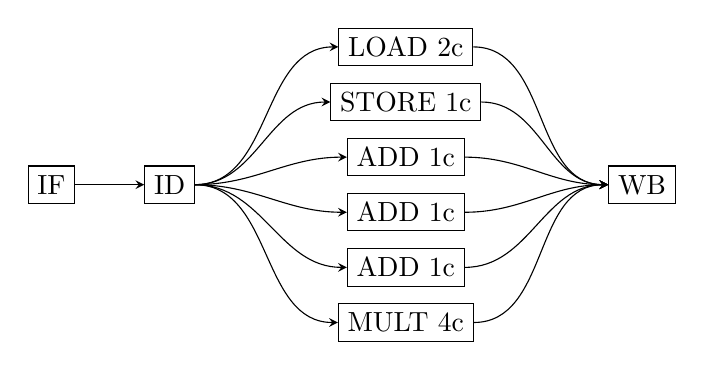
\begin{tikzpicture}
    \node[draw, rectangle] (A) at (-0.5,1.75) {IF};
    \node[draw, rectangle] (B) at (1,1.75) {ID};

    \node[draw, rectangle] (C) at (4,3.5) {LOAD 2c};
    \node[draw, rectangle] (D) at (4,2.8) {STORE 1c};
    \node[draw, rectangle] (E) at (4,2.1) {ADD 1c};
    \node[draw, rectangle] (F) at (4,1.4) {ADD 1c};
    \node[draw, rectangle] (G) at (4,0.7) {ADD 1c};
    \node[draw, rectangle] (H) at (4,0) {MULT 4c};

    \node[draw, rectangle] (I) at (7,1.75) {WB};

    \draw[-stealth] (A) -- (B);
    \draw[-stealth] (B) to[out=0,in=180] (C);
    \draw[-stealth] (B) to[out=0,in=180] (D);
    \draw[-stealth] (B) to[out=0,in=180] (E);
    \draw[-stealth] (B) to[out=0,in=180] (F);
    \draw[-stealth] (B) to[out=0,in=180] (G);
    \draw[-stealth] (B) to[out=0,in=180] (H);
    \draw[-stealth] (C) to[out=0,in=180] (I);
    \draw[-stealth] (D) to[out=0,in=180] (I);
    \draw[-stealth] (E) to[out=0,in=180] (I);
    \draw[-stealth] (F) to[out=0,in=180] (I);
    \draw[-stealth] (G) to[out=0,in=180] (I);
    \draw[-stealth] (H) to[out=0,in=180] (I);
\end{tikzpicture}
\end{figure}

Además, para cada caso, se ha desarrollado una tabla que muestra la evolución de la ejecución del código según el número de ciclos.

\begin{table}
\centering
\scriptsize
\begin{tabular}{|l|c|c|c|c|c|c|c|c|c|c|c|c|c|c|}
    \hline
    Instrucción / Ciclos & 1 & 2 & 3 & 4 & 5 & 6 & 7 & 8 & 9 & 10 & 11 & 12  & 13 & 14 \\
    \hline
    \verb|lw  r1, 0x1ac|     & IF & ID & EX & EX & & & & & & & & & & \\
    \hline        
    \verb|lw  r2, 0xc1f|     & IF & ID & & & EX & EX & & & & & & & & \\
    \hline           
    \verb|add r3, r0, r0|    & IF & ID & & & EX & & & & & & & & & \\
    \hline                        
    \verb|mul r4, r2, r1|    & IF & ID & & & & & EX & EX & EX & EX & & & & \\
    \hline            
    \verb|add r3, r3, r4|    & & IF & ID & & & & & & & & EX & & & \\
    \hline            
    \verb|add r5, r0, 0x1ac| & & IF & ID & & & & & & & & EX & & & \\
    \hline            
    \verb|add r6, r0, 0xc1f| & & IF & ID & & & & & & & & EX & & & \\
    \hline        
    \verb|sub r5, r5, #4|    & & IF & ID & & & & & & & & & EX & & \\
    \hline
    \verb|sub r6, r6, #4|    & & & IF & ID & & & & & & & & EX & & \\
    \hline
    \verb|sw  (r5), r3|      & & & IF & ID & & & & & & & & & EX & \\
    \hline          
    \verb|sw  (r6), r4|      & & & IF & ID & & & & & & & & & & EX \\
    \hline
\end{tabular}
\caption{Ejecución con ventana centralizada y emisión ordenada del Ejercicio~\ref{ej:1_R4}.}
\label{tab:ej1_R4_1}
\end{table}

\begin{table}
\centering
\scriptsize
\begin{tabular}{|l|c|c|c|c|c|c|c|c|c|c|c|c|}
    \hline
    Instrucción / Ciclos & 1 & 2 & 3 & 4 & 5 & 6 & 7 & 8 & 9 & 10 & 11 & 12  \\
    \hline
    \verb|lw  r1, 0x1ac|     & IF & ID & EX & EX & & & & & & & & \\
    \hline        
    \verb|lw  r2, 0xc1f|     & IF & ID & & & EX & EX & & & & & & \\
    \hline           
    \verb|add r3, r0, r0|    & IF & ID & EX & & & & & & & & & \\
    \hline                        
    \verb|mul r4, r2, r1|    & IF & ID & & & & & EX & EX & EX & EX & & \\
    \hline            
    \verb|add r3, r3, r4|    & & IF & ID & & & & & & & & EX & \\
    \hline
    \verb|add r5, r0, 0x1ac| & & IF & ID & EX & & & & & & & & \\
    \hline
    \verb|add r6, r0, 0xc1f| & & IF & ID & EX & & & & & & & & \\
    \hline
    \verb|sub r5, r5, #4|    & & IF & ID & & EX & & & & & & & \\
    \hline            
    \verb|sub r6, r6, #4|    & & & IF & ID & EX & & & & & & & \\
    \hline
    \verb|sw  (r5), r3|      & & & IF & ID & & & & & & &  & EX \\
    \hline
    \verb|sw  (r6), r4|      & & & IF & ID & & & & & & & EX &  \\
    \hline
\end{tabular}
\caption{Ventana centralizada y emisión desordenada del Ejercicio~\ref{ej:1_R4}.}
\label{tab:ej1_R4_2}
\end{table}

\begin{table}
\centering
\scriptsize
\begin{tabular}{|l|c|c|c|c|c|c|c|c|c|c|c|c|c|}
    \hline
    Instrucción / Ciclos & 1 & 2 & 3 & 4 & 5 & 6 & 7 & 8 & 9 & 10 & 11 & 12 & 13 \\
    \hline
    \verb|lw  r1, 0x1ac|     & IF & ID & EX & EX & & & & & & & & & \\
    \hline        
    \verb|lw  r2, 0xc1f|     & IF & ID & & & EX & EX & & & & & & & \\
    \hline           
    \verb|add r3, r0, r0| ~~(1)    & IF & ID & EX & & & & & & & & & & \\
    \hline                        
    \verb|mul r4, r2, r1|    & IF & ID & & & & & EX & EX & EX & EX & & & \\
    \hline            
    \verb|add r3, r3, r4| ~~(2)    & & IF & ID & & & & & & & & EX & & \\
    \hline
    \verb|add r5, r0, 0x1ac| ~~(3) & & IF & ID & EX & & & & & & & & & \\
    \hline
    \verb|add r6, r0, 0xc1f| ~~(1) & & IF & ID & EX & & & & & & & & & \\
    \hline
    \verb|sub r5, r5, #4| ~~(3)    & & IF & ID & & EX & & & & & & & & \\
    \hline            
    \verb|sub r6, r6, #4| ~~(1)    & & & IF & ID & EX & & & & & & & & \\
    \hline
    \verb|sw  (r5), r3|      & & & IF & ID & & & & & & & & EX & \\
    \hline
    \verb|sw  (r6), r4|      & & & IF & ID & & & & & & & & & EX \\
    \hline
\end{tabular}
\caption{Ejecución con ventanas repartidas y emisión ordenada del Ejercicio~\ref{ej:1_R4}.}
\label{tab:ej1_R4_3}
\end{table}

\end{ejercicio}

\begin{ejercicio}  \label{ej:2_R4}
    Cosidere el fragmento de Código~\ref{cod:ej2_R4}.
    \begin{listing}[H]
    \begin{minted}[xleftmargin=4cm, linenos]{asm}
lw   r3,0x10a   ; r3 <-- M(0x10a)
addi r2,r0,#128 ; r2 <-- r0+128
add  r1,r0,0x0a ; r1 <-- r0+0x0a
lw   r4,0(r1)   ; r4 <-- M(r1)
lw   r5,-8(r1)  ; r5 <-- M(r1-8)
mult r6,r5,r3   ; r6 <-- r5*r3
add  r5,r6,r3   ; r5 <-- r6+r3
add  r6,r4,r3   ; r6 <-- r4+r3
sw   0(r1),r6   ; M(r1) <-- r5
sw   -8(r1),r5  ; M(r1-8) <-- r5
sub  r2,r2,#16  ; r2 <-- r2-16
    \end{minted}
    \caption{Código para trabajar.}
    \label{cod:ej2_R4}
    \end{listing}
Suponga que se ejecuta en un procesador superescalar que es capaz de captar 4 instrucciones/ciclo, de decodificar 2 instrucciones/ciclo; de emitir utilizando una ventana de instrucciones centralizada 2 instrucciones/ciclo; de escribir hasta 2 resultados/ciclo en los registros correspondientes (registros de reorden, o registros de la arquitectura según el caso), y completar (o retirar) hasta 3 instrucciones/ciclo.

Indique el número de ciclos que tardaría en ejecutarse el programa suponiendo finalización ordenada y:
\begin{enumerate}
    \item Emisión ordenada.
    
    Se encuentra resuelto en la Tabla~\ref{tab:ej2_R4_1}.
    \item Emisión desordenada.
    
    Se encuentra resuelto en la Tabla~\ref{tab:ej2_R4_2}. Notemos que, como
    no pueden escribir en el ROB más de dos instrucciones por ciclo,
    la instrucción \verb|sub r2,r2,#16| ha de esperar un ciclo más.
\end{enumerate}
Nota: Considere que tiene una unidad funcional de carga (2 ciclos), una de almacenamiento (1 ciclo), tres unidades de suma/resta (1 ciclo), y una de multiplicación (6 ciclos), y que no hay limitaciones para el número de líneas de la cola de instrucciones, ventana de instrucciones, buffer de reorden, puertos de lectura/escritura etc.


Según el enunciado del ejercicio, el cauce de instrucciones tiene la siguiente forma:
\begin{figure}[H]
\centering
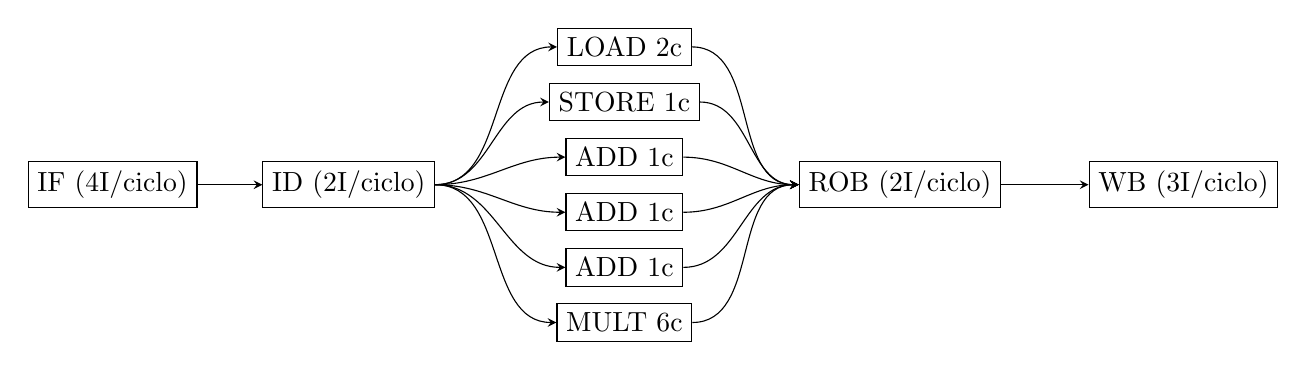
\begin{tikzpicture}
    \node[draw, rectangle] (A) at (-2.5,1.75) {IF (4I/ciclo)};
    \node[draw, rectangle] (B) at (00.5,1.75) {ID (2I/ciclo)};

    \node[draw, rectangle] (C) at (4,3.5) {LOAD 2c};
    \node[draw, rectangle] (D) at (4,2.8) {STORE 1c};
    \node[draw, rectangle] (E) at (4,2.1) {ADD 1c};
    \node[draw, rectangle] (F) at (4,1.4) {ADD 1c};
    \node[draw, rectangle] (G) at (4,0.7) {ADD 1c};
    \node[draw, rectangle] (H) at (4,0) {MULT 6c};

    \node[draw, rectangle] (I) at (7.5,1.75) {ROB (2I/ciclo)};
    \node[draw, rectangle] (J) at (11.1,1.75) {WB (3I/ciclo)};

    \draw[-stealth] (A) -- (B);
    \draw[-stealth] (B) to[out=0,in=180] (C);
    \draw[-stealth] (B) to[out=0,in=180] (D);
    \draw[-stealth] (B) to[out=0,in=180] (E);
    \draw[-stealth] (B) to[out=0,in=180] (F);
    \draw[-stealth] (B) to[out=0,in=180] (G);
    \draw[-stealth] (B) to[out=0,in=180] (H);
    \draw[-stealth] (C) to[out=0,in=180] (I);
    \draw[-stealth] (D) to[out=0,in=180] (I);
    \draw[-stealth] (E) to[out=0,in=180] (I);
    \draw[-stealth] (F) to[out=0,in=180] (I);
    \draw[-stealth] (G) to[out=0,in=180] (I);
    \draw[-stealth] (H) to[out=0,in=180] (I);
    \draw[-stealth] (I) to[out=0,in=180] (J);
\end{tikzpicture}
\end{figure}


\begin{table}
    \centering
    \scriptsize
    \begin{tabular}{|l|c|c|c|c|c|c|c|c|c|c|c|c|}
        \hline
        Instrucción / Ciclos & 1 & 2 & 3 & 4 & 5 & 6 & 7 & 8 & 9 & 10 & 11 & 12 \\
        \hline
        \verb|lw   r3,0x10a|        & IF & ID & EX & EX & ROB & WB & & & & & &\\
        \hline        
        \verb|addi r2,r0,#128|      & IF & ID & EX & ROB & & WB & & & & & &\\
        \hline           
        \verb|add  r1,r0,0x0a|      & IF & & ID & EX & ROB & WB & & & & & &\\
        \hline                        
        \verb|lw   r4,0(r1)|        & IF & & ID & & EX & EX & ROB & WB & & & &\\
        \hline            
        \verb|lw   r5,-8(r1)|       & & IF & & ID & & & EX & EX & ROB & WB & &\\
        \hline
        \verb|mult r6,r5,r3|        & & IF & & ID & & & & & EX & EX & EX & EX \\
        \hline
        \verb|add  r5,r6,r3|        & & IF & & & ID & & & & & & &\\
        \hline
        \verb|add  r6,r4,r3|        & & IF & & & ID & & & & & & &\\
        \hline            
        \verb|sw   0(r1),r6|        & & & IF & & & ID & & & & & &\\
        \hline
        \verb|sw  -8(r1),r5|        & & & IF & & & ID & & & & & &\\
        \hline
        \verb|sub  r2,r2,#16|       & & & IF & & & & ID & & & & &\\
        \hline \\ \hline \\ \hline
        \hline
        Instrucción / Ciclos & 13 & 14 & 15 & 16 & 17 & 18 & 19 \\
        \hline
        \verb|lw   r3,0x10a|        & & & & & & &\\
        \hline        
        \verb|addi r2,r0,#128|      & & & & & & &\\
        \hline           
        \verb|add  r1,r0,0x0a|      & & & & & & &\\
        \hline                        
        \verb|lw   r4,0(r1)|        & & & & & & &\\
        \hline            
        \verb|lw   r5,-8(r1)|       & & & & & & &\\
        \hline
        \verb|mult r6,r5,r3|        & EX & EX & ROB & WB & & & \\
        \hline
        \verb|add  r5,r6,r3|        & & & EX & ROB & WB & & \\
        \hline
        \verb|add  r6,r4,r3|        & & & EX & ROB & WB & & \\
        \hline            
        \verb|sw   0(r1),r6|        & & & & EX & ROB & WB & \\
        \hline
        \verb|sw  -8(r1),r5|        & & & & & EX & ROB & WB \\
        \hline
        \verb|sub  r2,r2,#16|       & & & & & EX & ROB & WB\\
        \hline
    \end{tabular}
    \caption{Emisión ordenada del código del Ejercicio~\ref{ej:2_R4}.}
    \label{tab:ej2_R4_1}
\end{table}

\begin{table}
    \centering
    \scriptsize
    \begin{tabular}{|l|c|c|c|c|c|c|c|c|c|c|c|c|}
        \hline
        Instrucción / Ciclos & 1 & 2 & 3 & 4 & 5 & 6 & 7 & 8 & 9 & 10 & 11 & 12 \\
        \hline
        \verb|lw   r3,0x10a|        & IF & ID & EX & EX & ROB & WB & & & & & &\\
        \hline        
        \verb|addi r2,r0,#128|      & IF & ID & EX & ROB & & WB & & & & & &\\
        \hline           
        \verb|add  r1,r0,0x0a|      & IF & & ID & EX & ROB & WB & & & & & &\\
        \hline                        
        \verb|lw   r4,0(r1)|        & IF & & ID & & EX & EX & ROB & WB & & & &\\
        \hline            
        \verb|lw   r5,-8(r1)|       & & IF & & ID & & & EX & EX & ROB & WB & &\\
        \hline
        \verb|mult r6,r5,r3|        & & IF & & ID & & & & & EX & EX & EX & EX \\
        \hline
        \verb|add  r5,r6,r3|        & & IF & & & ID & & & & & & &\\
        \hline
        \verb|add  r6,r4,r3|        & & IF & & & ID & & EX & ROB & & & &\\
        \hline            
        \verb|sw   0(r1),r6|        & & & IF & & & ID & & EX & ROB & & &\\
        \hline
        \verb|sw  -8(r1),r5|        & & & IF & & & ID & & & & & &\\
        \hline
        \verb|sub  r2,r2,#16|       & & & IF & & & & ID & EX & & \red{ROB} & &\\
        \hline \\ \hline \\ \hline
        \hline
        Instrucción / Ciclos & 13 & 14 & 15 & 16 & 17 & 18 & 19 \\
        \hline
        \verb|lw   r3,0x10a|        & & & & & & &\\
        \hline        
        \verb|addi r2,r0,#128|      & & & & & & &\\
        \hline           
        \verb|add  r1,r0,0x0a|      & & & & & & &\\
        \hline                        
        \verb|lw   r4,0(r1)|        & & & & & & &\\
        \hline            
        \verb|lw   r5,-8(r1)|       & & & & & & &\\
        \hline
        \verb|mult r6,r5,r3|        & EX & EX & ROB & WB & & & \\
        \hline
        \verb|add  r5,r6,r3|        & & & EX & ROB & WB & & \\
        \hline
        \verb|add  r6,r4,r3|        & & & & & \red{WB} & & \\
        \hline            
        \verb|sw   0(r1),r6|        & & & & & WB & & \\
        \hline
        \verb|sw  -8(r1),r5|        & & & & EX & ROB & WB & \\
        \hline
        \verb|sub  r2,r2,#16|       & & & & & & WB & \\
        \hline
    \end{tabular}
    \caption{Emisión desordenada del código del Ejercicio~\ref{ej:2_R4}.}
    \label{tab:ej2_R4_2}
\end{table}

\end{ejercicio}

\begin{ejercicio}\label{ej:3_R4}
   En el problema anterior: 
   \begin{enumerate}
       \item Indique qué mejoras realizaría en el procesador para reducir el tiempo de ejecución en la mejor de las opciones sin cambiar el diseño de las unidades funcionales (multiplicador, sumador, etc.) y sin cambiar el tipo de memorias ni la interfaz entre procesador y memoria (no varía el número de instrucciones captadas por ciclo).
       
       En primer lugar, consideramos que se decodifican el mismo número de instrucciones que se captan,
       eliminante el cuello de botella en la decodificación que teníamos en el problema anterior.
       Además, consideramos que no hay límite en el número de instrucciones por ciclo que se emiten, escriben en el ROB o completan.
       Por último, consideramos que disponemos de tantas unidades funcionales como se necesiten, para evitar así riesgos estructurales.
       Con estas mejoras, hemos llegado a la tabla~\ref{tab:ej3_R4_1}.
       
       \item ¿Qué pasaría si además se reduce el tiempo de multiplicación a la mitad?
       
       Resuelto en la tabla~\ref{tab:ej3_R4_2}. En este caso, tenemos una latencia inicial de $6$
       ciclos de reloj. Sabiendo que se ejecutan $11$ instrucciones en $12$ ciclos de reloj,
       tenemos que:
       \begin{equation*}
        T(n) = 12 = TLI + (n-1)CPI = 6 + (11-1)CPI \Rightarrow CPI = \frac{12-6}{11-1} = \frac{6}{10} = 0.6
       \end{equation*}

       Como $CPI=0.6<1$, podemos decir que el procesador es superescalar, pero no se trata de su
       mejor versión, ya que podemos llegar incluso a $3$ instrucciones por ciclo.
   \end{enumerate}
   
    \begin{table}
        \centering
        \scriptsize
        \begin{tabular}{|l|c|c|c|c|c|c|c|c|c|c|c|c|}
            \hline
            Instrucción / Ciclos & 1 & 2 & 3 & 4 & 5 & 6 & 7 & 8 & 9 & 10 & 11 & 12 \\
            \hline
            \verb|lw   r3,0x10a|        & IF & ID & EX & EX & ROB & WB & & & & & &\\
            \hline        
            \verb|addi r2,r0,#128|      & IF & ID & EX & ROB & & WB & & & & & &\\
            \hline           
            \verb|add  r1,r0,0x0a|      & IF & ID & EX & ROB & &  WB & & & & & & \\
            \hline                        
            \verb|lw   r4,0(r1)|        & IF & ID & & EX & EX & ROB & WB & & & & & \\
            \hline            
            \verb|lw   r5,-8(r1)|       & & IF & ID & EX & EX & ROB & WB & & & && \\
            \hline
            \verb|mult r6,r5,r3|        & & IF & ID & & & EX & EX & EX & EX & EX & EX & ROB\\
            \hline
            \verb|add  r5,r6,r3|        & & IF & ID & & & & & & & & & EX\\
            \hline
            \verb|add  r6,r4,r3|        & & IF & ID & & & EX & ROB & & & & &\\
            \hline            
            \verb|sw   0(r1),r6|        & & & IF & ID & & & EX & ROB & & & & \\
            \hline
            \verb|sw  -8(r1),r5|        & & & IF & ID & & & & & & & &\\
            \hline
            \verb|sub  r2,r2,#16|       & & & IF & ID & EX & ROB & & & & & & \\
            \hline \\ \hline \\ \hline
            \hline
            Instrucción / Ciclos & 13 & 14 & 15 & 16 & 17 & 18 & 19 \\
            \hline
            \verb|lw   r3,0x10a|        & & & & & & &\\
            \hline        
            \verb|addi r2,r0,#128|      & & & & & & &\\
            \hline           
            \verb|add  r1,r0,0x0a|      & & & & & & &\\
            \hline                        
            \verb|lw   r4,0(r1)|        & & & & & & &\\
            \hline            
            \verb|lw   r5,-8(r1)|       & & & & & & &\\
            \hline
            \verb|mult r6,r5,r3|        & WR & & & & & & \\
            \hline
            \verb|add  r5,r6,r3|        & ROB & WB & & & & &\\
            \hline
            \verb|add  r6,r4,r3|        & & WB & & & & & \\
            \hline            
            \verb|sw   0(r1),r6|        & & WB & & & & & \\
            \hline
            \verb|sw  -8(r1),r5|        & EX & ROB & WB & & & & \\
            \hline
            \verb|sub  r2,r2,#16|       & & & WB & & & & \\
            \hline
        \end{tabular}
        \caption{Emisión desordenada del código de las mejoras Ejercicio~\ref{ej:2_R4}.}
        \label{tab:ej3_R4_1}
    \end{table}

    \begin{table}
        \centering
        \scriptsize
        \begin{tabular}{|l|c|c|c|c|c|c|c|c|c|c|c|c|}
            \hline
            Instrucción / Ciclos & 1 & 2 & 3 & 4 & 5 & 6 & 7 & 8 & 9 & 10 & 11 & 12 \\
            \hline
            \verb|lw   r3,0x10a|        & IF & ID & EX & EX & ROB & WB & & & & & &\\
            \hline        
            \verb|addi r2,r0,#128|      & IF & ID & EX & ROB & & WB & & & & & &\\
            \hline           
            \verb|add  r1,r0,0x0a|      & IF & ID & EX & ROB & &  WB & & & & & & \\
            \hline                        
            \verb|lw   r4,0(r1)|        & IF & ID & & EX & EX & ROB & WB & & & & & \\
            \hline            
            \verb|lw   r5,-8(r1)|       & & IF & ID & EX & EX & ROB & WB & & & && \\
            \hline
            \verb|mult r6,r5,r3|        & & IF & ID & & & EX & EX & EX & ROB & WR & & \\
            \hline
            \verb|add  r5,r6,r3|        & & IF & ID & & & & & & EX & ROB & WR & \\
            \hline
            \verb|add  r6,r4,r3|        & & IF & ID & & & EX & ROB & & & & WR &\\
            \hline            
            \verb|sw   0(r1),r6|        & & & IF & ID & & & EX & ROB & & & WR & \\
            \hline
            \verb|sw  -8(r1),r5|        & & & IF & ID & & & & & & EX & ROB & WB\\
            \hline
            \verb|sub  r2,r2,#16|       & & & IF & ID & EX & ROB & & & & & & WB \\
            \hline
        \end{tabular}
        \caption{Emisión desordenada reduciendo la multiplicación del Ejercicio~\ref{ej:2_R4}.}
        \label{tab:ej3_R4_2}
    \end{table}
\end{ejercicio}

\begin{ejercicio}
    En el caso descrito en el problema~\ref{ej:3_R4}, indique cómo evolucionaría el buffer de reorden utilizado para implementar finalización ordenada, en la mejor de las opciones.

    En todo momento, nos referiremos a la tabla~\ref{tab:ej3_R4_2} para describir la evolución del buffer de reorden, ya que es la que da mejores resultados.
    Tras terminar el ciclo $1$, tan solo se han captado instrucciones, pero todavía no se han decodificado las instrucciones ni se han emitido (que es el momento en el que se añaden al buffer de reorden).
    Por tanto, en este momento dicho buffer está vacío. Tras terminar el ciclo $2$, se añaden las 4 instrucciones emitidas:
    \begin{center}
        \scriptsize
        \begin{tabular}{|c|c|c|c|c|c|c|c|c|}
            \hline
            \multicolumn{8}{|c|}{Ciclo 2} \\
            \hline
            \# & Codop      & Unidad & Destino & Valor & Válido & Último & Marca \\ \hline
            0  & \verb|lw|  & LOAD   & r3      &       & 0      & 1      & i     \\ \hline
            1  & \verb|addi|& ADD    & r2      &       & 0      & 1      & i     \\ \hline
            2  & \verb|add| & ADD    & r1      &       & 0      & 1      & i     \\ \hline
            3  & \verb|lw|  & LOAD   & r4      &       & 0      & 1      & i     \\ \hline
        \end{tabular}
    \end{center}

    En el ciclo $3$, otras 4 instrucciones se decodifican y se emiten, y de las que ya estaban emitidas tres entran a la etapa de ejecución. Expresamos ya
    todos los ciclos a continuación, teniendo en cuenta que la marca \verb|f| se escribe en la etapa ROB.
    \begin{center}
        \scriptsize
        \begin{tabular}{|c|c|c|c|c|c|c|c|c|}
            \hline
            \multicolumn{8}{|c|}{Ciclo 3} \\
            \hline
            \# & Codop      & Unidad & Destino & Valor & Válido & Último & Marca \\ \hline
            0  & \verb|lw|  & LOAD   & r3      &       & 0      & 1      & x     \\ \hline
            1  & \verb|addi|& ADD    & r2      &       & 0      & 1      & x     \\ \hline
            2  & \verb|add| & ADD    & r1      &       & 0      & 1      & x     \\ \hline
            3  & \verb|lw|  & LOAD   & r4      &       & 0      & 1      & i     \\ \hline
            4  & \verb|lw|  & LOAD   & r5      &       & 0      & 0      & i     \\ \hline
            5  & \verb|mult|& MULT   & r6      &       & 0      & 0      & i     \\ \hline
            6  & \verb|add| & ADD    & r5      &       & 0      & 1      & i     \\ \hline
            7  & \verb|add| & ADD    & r6      &       & 0      & 1      & i     \\ \hline
            \hline
            \multicolumn{8}{|c|}{Ciclo 4} \\
            \hline
            \# & Codop      & Unidad & Destino & Valor & Válido & Último & Marca \\ \hline
            0  & \verb|lw|  & LOAD   & r3      &       & 0      & 1      & x     \\ \hline
            1  & \verb|addi|& ADD    & r2      & [r0+\#128] & 1 & 0      & f     \\ \hline
            2  & \verb|add| & ADD    & r1      & [r0+0x0A]  & 1 & 1      & f     \\ \hline
            3  & \verb|lw|  & LOAD   & r4      &       & 0      & 1      & x     \\ \hline
            4  & \verb|lw|  & LOAD   & r5      &       & 0      & 0      & x     \\ \hline
            5  & \verb|mult|& MULT   & r6      &       & 0      & 0      & i     \\ \hline
            6  & \verb|add| & ADD    & r5      &       & 0      & 1      & i     \\ \hline
            7  & \verb|add| & ADD    & r6      &       & 0      & 1      & i     \\ \hline
            8  & \verb|sw|  & STORE  & -       &       & 0      & 1      & i     \\ \hline
            9  & \verb|sw|  & STORE  & -       &       & 0      & 1      & i     \\ \hline
            10 & \verb|sub| & ADD    & r2      &       & 0      & 1      & i     \\ \hline
        \end{tabular}
        \end{center}

    \begin{table}[H]
        \centering
        \scriptsize
        \begin{tabular}{|c|c|c|c|c|c|c|c|c|}
            \hline
            \multicolumn{8}{|c|}{Ciclo 5} \\
            \hline
            \# & Codop      & Unidad & Destino & Valor & Válido & Último & Marca \\ \hline
            0  & \verb|lw|  & LOAD   & r3      &  M[0x10a]  & 1 & 1      & f     \\ \hline
            1  & \verb|addi|& ADD    & r2      & [r0+\#128] & 1 & 0      & f     \\ \hline
            2  & \verb|add| & ADD    & r1      & [r0+0x0A]  & 1 & 1      & f     \\ \hline
            3  & \verb|lw|  & LOAD   & r4      &       & 0      & 1      & x     \\ \hline
            4  & \verb|lw|  & LOAD   & r5      &       & 0      & 0      & x     \\ \hline
            5  & \verb|mult|& MULT   & r6      &       & 0      & 0      & i     \\ \hline
            6  & \verb|add| & ADD    & r5      &       & 0      & 1      & i     \\ \hline
            7  & \verb|add| & ADD    & r6      &       & 0      & 1      & i     \\ \hline
            8  & \verb|sw|  & STORE  & -       &       & 0      & 1      & i     \\ \hline
            9  & \verb|sw|  & STORE  & -       &       & 0      & 1      & i     \\ \hline
            10 & \verb|sub| & ADD    & r2      &       & 0      & 1      & x     \\ \hline\hline
            \multicolumn{8}{|c|}{Ciclo 6} \\
            \hline
            \# & Codop      & Unidad & Destino & Valor & Válido & Último & Marca \\ \hline
            3  & \verb|lw|  & LOAD   & r4      & M[r1] & 1      & 1      & f     \\ \hline
            4  & \verb|lw|  & LOAD   & r5      & M[-8(ri)] & 1  & 0      & f     \\ \hline
            5  & \verb|mult|& MULT   & r6      &       & 0      & 0      & x     \\ \hline
            6  & \verb|add| & ADD    & r5      &       & 0      & 1      & i     \\ \hline
            7  & \verb|add| & ADD    & r6      &       & 0      & 1      & x     \\ \hline
            8  & \verb|sw|  & STORE  & -       &       & 0      & 1      & i     \\ \hline
            9  & \verb|sw|  & STORE  & -       &       & 0      & 1      & i     \\ \hline
            10 & \verb|sub| & ADD    & r2      & [r2-\#16] & 1  & 1      & f     \\ \hline\hline
            \multicolumn{8}{|c|}{Ciclo 7} \\
            \hline
            \# & Codop      & Unidad & Destino & Valor & Válido & Último & Marca \\ \hline
            5  & \verb|mult|& MULT   & r6      &       & 0      & 0      & x     \\ \hline
            6  & \verb|add| & ADD    & r5      &       & 0      & 1      & i     \\ \hline
            7  & \verb|add| & ADD    & r6      & [r4+r3]  & 1   & 1      & f     \\ \hline
            8  & \verb|sw|  & STORE  & -       &       & 0      & 1      & x     \\ \hline
            9  & \verb|sw|  & STORE  & -       &       & 0      & 1      & i     \\ \hline
            10 & \verb|sub| & ADD    & r2      & [r2-\#16] & 1  & 1      & f     \\ \hline\hline
            \multicolumn{8}{|c|}{Ciclo 8} \\
            \hline
            \# & Codop      & Unidad & Destino & Valor & Válido & Último & Marca \\ \hline
            5  & \verb|mult|& MULT   & r6      &       & 0      & 0      & x     \\ \hline
            6  & \verb|add| & ADD    & r5      &       & 0      & 1      & i     \\ \hline
            7  & \verb|add| & ADD    & r6      & [r4+r3]  & 1   & 1      & f     \\ \hline
            8  & \verb|sw|  & STORE  & -       & -     & 0      & 1      & f     \\ \hline
            9  & \verb|sw|  & STORE  & -       &       & 0      & 1      & i     \\ \hline
            10 & \verb|sub| & ADD    & r2      & [r2-\#16] & 1  & 1      & f     \\ \hline\hline
            \multicolumn{8}{|c|}{Ciclo 9} \\
            \hline
            \# & Codop      & Unidad & Destino & Valor & Válido & Último & Marca \\ \hline
            5  & \verb|mult|& MULT   & r6      & [r5*r3] & 1    & 0      & f     \\ \hline
            6  & \verb|add| & ADD    & r5      &       & 0      & 1      & x     \\ \hline
            7  & \verb|add| & ADD    & r6      & [r4+r3]  & 1   & 1      & f     \\ \hline
            8  & \verb|sw|  & STORE  & -       &  -    & 0      & 1      & f     \\ \hline
            9  & \verb|sw|  & STORE  & -       &       & 0      & 1      & i     \\ \hline
            10 & \verb|sub| & ADD    & r2      & [r2-\#16] & 1  & 1      & f     \\ \hline\hline
            \multicolumn{8}{|c|}{Ciclo 10} \\
            \hline
            \# & Codop      & Unidad & Destino & Valor & Válido & Último & Marca \\ \hline
            6  & \verb|add| & ADD    & r5      & [r6+r3] & 0    & 1      & f     \\ \hline
            7  & \verb|add| & ADD    & r6      & [r4+r3] & 0    & 1      & f     \\ \hline
            8  & \verb|sw|  & STORE  & -       & -     & 0      & 1      & f     \\ \hline
            9  & \verb|sw|  & STORE  & -       &       & 0      & 1      & x     \\ \hline
            10 & \verb|sub| & ADD    & r2      & [r2-\#16] & 1  & 1      & f     \\ \hline\hline
            \multicolumn{8}{|c|}{Ciclo 11} \\
            \hline
            \# & Codop      & Unidad & Destino & Valor & Válido & Último & Marca \\ \hline
            9  & \verb|sw|  & STORE  & -       & -     & 0      & 1      & f     \\ \hline
            10 & \verb|sub| & ADD    & r2      & [r2-\#16] & 1  & 1      & f     \\ \hline\hline
            \multicolumn{8}{|c|}{Ciclo 12} \\
            \hline
            \# & Codop      & Unidad & Destino & Valor & Válido & Último & Marca \\ \hline
            \multicolumn{8}{|c|}{} \\
            \hline
        \end{tabular}
    \end{table}
\end{ejercicio}

\begin{ejercicio}
    En un procesador superescalar con renombramiento de registros se utiliza un buffer de renombramiento para implementar el mismo. Indique como evolucionarían los registros de renombramiento al realizar el renombramiento para las instrucciones del Código~\ref{cod:e5_R4}.
    \begin{listing}[H]
    \begin{minted}[xleftmargin=4cm, linenos]{asm}
mul r2, r0, r1  ; r2 <-- r0*r1
add r3,r1,r2    ; r3 <-- r1+r2
sub r2,r0,r1    ; r2 <-- r0-r1
add r3,r3,r2    ; r3 <-- r3+r2
    \end{minted}
    \caption{Instrucciones para renombrar.}
    \label{cod:e5_R4}
    \end{listing}

    Suponemos que \verb|r0| y \verb|r1| ya se encuentran en el buffer de renombramiento, siendo este inicialmente como sigue:
    \begin{center}
        \scriptsize
        \begin{tabular}{|c|c|c|c|c|c|}
            \hline
            \# & Entrada Válida & Registro destino & Valor & Válido & Último \\
            \hline
            0 & 1 & r0 & [r0] & 1 & 1 \\
            1 & 1 & r1 & [r1] & 1 & 1 \\
            \hline
        \end{tabular}
    \end{center}

    Tras decodificar la primera instrucción, \verb|mul r2, r0, r1|, el buffer de renombramiento queda como sigue:
    \begin{center}
        \scriptsize
        \begin{tabular}{|c|c|c|c|c|c|}
            \hline
            \# & Entrada Válida & Registro destino & Valor & Válido & Último \\
            \hline
            0 & 1 & r0 & [r0] & 1 & 1 \\
            1 & 1 & r1 & [r1] & 1 & 1 \\
            2 & 1 & r2 &  & 0 & 1 \\
            \hline
        \end{tabular}
    \end{center}

    Tras decodificar la segunda instrucción, \verb|add r3,r1,r2|, el buffer de renombramiento queda como sigue:
    \begin{center}
        \scriptsize
        \begin{tabular}{|c|c|c|c|c|c|}
            \hline
            \# & Entrada Válida & Registro destino & Valor & Válido & Último \\
            \hline
            0 & 1 & r0 & [r0] & 1 & 1 \\
            1 & 1 & r1 & [r1] & 1 & 1 \\
            2 & 1 & r2 &  & 0 & 1 \\
            3 & 1 & r3 &  & 0 & 1 \\
            \hline
        \end{tabular}
    \end{center}

    Notemos que esta última instrucción no puede completarse hasta que la primera no lo haya hecho, ya que \verb|r2| no se encuentra en el buffer de renombramiento.
    Estará por tanto esperando en la estación de reserva hasta que se complete la primera instrucción. Tras la captación de la tercera instrucción, \verb|sub r2,r0,r1|, el buffer de renombramiento queda como sigue:
    \begin{center}
        \scriptsize
        \begin{tabular}{|c|c|c|c|c|c|}
            \hline
            \# & Entrada Válida & Registro destino & Valor & Válido & Último \\
            \hline
            0 & 1 & r0 & [r0] & 1 & 1 \\
            1 & 1 & r1 & [r1] & 1 & 1 \\
            2 & 1 & r2 &  & 0 & 0 \\
            3 & 1 & r3 &  & 0 & 1 \\
            4 & 1 & r2 &  & 0 & 1 \\
            \hline
        \end{tabular}
    \end{center}

    Como \verb|r0| y \verb|r1| tienen valores válidos, esta instrucción podría empezar a ejecutarse si existe una unidad funcional
    disponible. El resultado de esta operación se almacenará en la línea 4 (último renombrado de \verb|r2|) y de ahí se
    tomarán los operandos \verb|r2| en instrucciones posteriores (para eso se utiliza el ``Bit de Último'').
    No obstante, supongamos que esta no se ejecuta todavía (por ejemplo, se podrián decodificar 4 instrucciones a la vez). Tras la decodificación de la última instrucción, \verb|add r3,r3,r2|, el buffer de renombramiento queda como sigue:
    \begin{center}
        \scriptsize
        \begin{tabular}{|c|c|c|c|c|c|}
            \hline
            \# & Entrada Válida & Registro destino & Valor & Válido & Último \\
            \hline
            0 & 1 & r0 & [r0] & 1 & 1 \\
            1 & 1 & r1 & [r1] & 1 & 1 \\
            2 & 1 & r2 &  & 0 & 0 \\
            3 & 1 & r3 &  & 0 & 0 \\
            4 & 1 & r2 &  & 0 & 1 \\
            5 & 1 & r3 &  & 0 & 1 \\
            \hline
        \end{tabular}
    \end{center}

    Cuando la instrucción \verb|mull r2,r0,r1| se complete, se actualizará la línea 2 con el valor de \verb|r2|,
    de forma que la instrucción \verb|add r3,r1,r2| pueda completarse. Cuando además se termine la instrucción \verb|sub r2,r0,r1|, se actualizará la línea 3 con el valor de \verb|r2|, de forma que la instrucción \verb|add r3,r3,r2|
    ya pueda completarse.
\end{ejercicio}

\begin{ejercicio}\label{ej:6_R4}
    Considere el bucle del Código~\ref{cod:ej6_R4}.
    \begin{listing}[H]
    \begin{minted}[xleftmargin=4cm, linenos]{c}
i=1;
do
{
    b[i]=a[i]*c;
    c=c+1;
    if (c>10) then goto etiqueta; // 1
    i=i+1;
} while (i<=10); // 2
etiqueta: //..
    \end{minted}
    \caption{Bucle a considerar.}
    \label{cod:ej6_R4}
    \end{listing}

Indique cuál es la penalización efectiva debida a los saltos, en función del valor inicial de \verb|c| (número entero). Considere que la penalización por saltos incorrectamente predichos es de 4 ciclos y para los saltos correctamente predichos es 0 ciclos. Diferencie según el procesador utilice:
\begin{enumerate}
    \item Predicción fija (siempre se considera que se va a producir el salto).
    
    Distinguimos en función del valor de \verb|c|, sabiendo que como mucho se van a realizar 10 iteraciones del bucle.
    \begin{itemize}
        \item Si \verb|c <= 0|:
        
        En este caso, por cada iteración del bucle, se va a producir un error de predicción,
        puesto que en ningún caso saltará. Por último, cuando sea \verb|i==10|, se predecirá saltar, lo que será un error. Por tanto,
        en total se producen $11$ predicciones fallidas, por lo que la penalización es de $44$ ciclos.

        \item Si \verb|c >= 10|:
        
        En este caso, se predecirá saltar cuando se llegue a la línea 6, y se acertara, terminando entonces el programa. Por tanto,
        no se producirá penalización ninguna.

        \item Si \verb|0<c<10|:
        
        En este caso, el salto etiquetado como $2$ nunca producirá penalización, porque siempre se saltará y nunca se llegará a \verb|i==10|.
        Se producirán $10-c$ errores de predicción, por lo que la penalización será de $4(10-c)$ ciclos.
    \end{itemize}

    \item Predicción estática según desplazamiento.
    
    \begin{itemize}
        \item Si \verb|c <= 0|:
        
        En este caso, en cada iteración del bucle, como el salto $1$ es hacia delante, se predecirá no saltar, acertando en la predicción.
        Además, en cada iteración se predecirá también de forma correcta saltar hacia atrás para volver a comenzar el bucle. Tan solo se producirá error
        en la última iteración, donde se tenga que terminar el bucle y se prediga saltar hacia atrás. Por tanto,
        tan solo se producirá un error de predicción; es decir, una penalización de 4 ciclos.

        \item Si \verb|c >= 10|:
        
        En este caso, como el salto $1$ es hacia delante, se predecirá no saltar, cuando en realidad sí se produce el salto. Por tanto,
        se trata de un error de predicción, que supone 4 ciclos de penalización.

        \item Si \verb|0<c<10|:
        
        En este caso, el salto etiquetado como $2$ nunca producirá penalización, porque siempre se saltará y es lo que se predice por ser un salto hacia detrás.
        Asimismo, el salto $1$ tan solo producirá error de predicción cuando se llegue a \verb|c==11|, que es cuando, aunque habiendo predicho que no se salte por ser un salto hacia delante,
        se saltará. Por tanto, el coste es de $4$ ciclos.
    \end{itemize}

    \item Predicción dinámica con un bit (Inicialmente está a 1).
    
    En este caso, necesitamos la Tabla de Saltos. Distinguimos en función del valor de \verb|c|, sabiendo que como mucho se van a realizar 10 iteraciones del bucle.
    \begin{itemize}
        \item Si \verb|c <= 0|:
        
        La Tabla de Saltos, en cada iteración del bucle, se actualizará de la siguiente forma:
        \begin{center}
            \begin{tabular}{|c|c|c|c|c|c|c|c|c|c|c|c|}
                \hline
                \# & Init. & It. 1& It. 2 & It. 3 & It. 4 & It. 5 & It. 6 & It. 7 & It. 8 & It. 9 & It. 10 \\ 
                \hline
                1 & 1 & 0 & 0 & 0 & 0 & 0 & 0 & 0 & 0 & 0 & 0\\
                2 & 1 & 1 & 1 & 1 & 1 & 1 & 1 & 1 & 1 & 1 & 0\\
                \hline \hline
                & & 1 err & & & & & & & & & 1 err \\
                \hline
            \end{tabular}
        \end{center}

        En este caso, se producen dos errores de predicción, uno en la primera iteración en el salto 1 y otro en la última en el salto 2, por lo que la penalización es de $8$ ciclos.

        \item Si \verb|c >= 10|:
        
        La Tabla de Saltos, en cada iteración del bucle, se actualizará de la siguiente forma:
        \begin{center}
            \begin{tabular}{|c|c|c|c|c|c|c|c|c|c|c|c|}
                \hline
                \# & Init. & It. 1& It. 2 & It. 3 & It. 4 & It. 5 & It. 6 & It. 7 & It. 8 & It. 9 & It. 10 \\ 
                \hline
                1 & 1 & 1 & - & - & - & - & - & - & - & - & -\\
                2 & 1 & - & - & - & - & - & - & - & - & - & -\\
                \hline \hline
                & & & & & & & & & & &\\
                \hline
            \end{tabular}
        \end{center}

        Notemos que en la primera iteración, se produce correctamente saltar, por lo que se termina el bucle. Por tanto, no se produce penalización alguna, y los
        guiones se han empleado para indicar que no se ejecutan más iteraciones.

        \item Si \verb|0<c<10|:
        
        En este caso, se realizarán $10-c$ 
        
        la Tabla de Saltos, en cada iteración del bucle, se actualizará de la siguiente forma:
        \begin{center}
            \begin{tabular}{|c|c|c|c|c|c|c|c|c|}
                \hline
                \# & Init. & It. 1& It. 2 & \dots & It. $10-c-1$ & It. $10-c$ & \dots & It. 10\\
                \hline
                1 & 1 & 0 & 0 & \dots & 0 & 1 & - & - \\
                2 & 1 & 1 & 1 & \dots & 1 & 1 & - & - \\
                \hline \hline
                & & 1 err & & & & 1 err & &\\
                \hline
            \end{tabular}
        \end{center}

        En este caso, se producen dos errores de predicción, uno en la primera iteración en el salto 1 y otro en la última iteración en el mismo salto, por lo que la penalización es de $8$ ciclos.
    \end{itemize}
\end{enumerate}
\end{ejercicio}

\begin{ejercicio}
    En la situación descrita en el problema~\ref{ej:6_R4}. ¿Cuál de los tres esquemas es más eficaz por término medio si hay un 25\% de probabilidades de que \verb|c| sea menor o igual a 0, un 30\% de que sea mayor o igual a 10; y un 45\% de que sea cualquier número entre 1 y 9, siendo todos equiprobables?\\

    Distinguimos en función de cada uno de los tipos de predicciones:
    \begin{itemize}
        \item Predicción fija:
        
        La penalización media es de:
        \begin{equation*}
            P_{\text{fija}} = 0.25\cdot 44 + 0.45\cdot \dfrac{\sum_{i=1}^9(10-c)\cdot 4}{9} + 0.30\cdot 0 = \unit[20]{ciclos}
        \end{equation*}

        \item Predicción estática según desplazamiento:
        
        La penalización media es de:
        \begin{equation*}
            P_{\text{estática}} = 0.25\cdot 4 + 0.45\cdot \dfrac{\sum_{i=1}^9 4}{9} + 0.30\cdot 4 = \unit[4]{ciclos}
        \end{equation*}

        \item Predicción dinámica con un bit:
        
        La penalización media es de:
        \begin{equation*}
            P_{\text{dinámica}} = 0.25\cdot 8 + 0.45\cdot \dfrac{\sum_{i=1}^9 8}{9} + 0.30\cdot 0 = \unit[5.6]{ciclos}
        \end{equation*}
    \end{itemize}

    Como se puede ver, para este bucle, y para la distribución de probabilidad de los valores de \verb|c|, el esquema de
    predicción más eficiente corresponde a la predicción estática.
    En cualquier caso, esta situación depende de las probabilidades de los distintos valores de \verb|c|.
\end{ejercicio}

\begin{ejercicio}
En un programa, una instrucción de salto condicional (a una dirección de salto anterior) dada tiene el siguiente comportamiento en una ejecución de dicho programa:    
\begin{equation*}
    SSNNNSSNSNSNSSSSSN
\end{equation*}
donde $S$ indica que se produce el salto y N que no. Indique la penalización efectiva (teniendo en cuenta que la penalización por saltos incorrectamente predichos es de 5 ciclos y para los saltos correctamente predichos es 0 ciclos) que se introduce si se utiliza:
\begin{enumerate}
    \item Predicción fija (siempre se considera que se no se va a producir el salto).
    
    Tenemos que el número de errores producidos es igual al número de veces que sí se salta, que es de 11 veces. Por tanto, la penalización es de $11\cdot 5 = 55$ ciclos.
    \item Predicción estática según desplazamiento.
    
    Como el salto es hacia atrás, siempre se predice que se va a saltar.
    Por tanto, el número de errores producidos es igual al número de veces que no se salta, que es de 7 veces. Por tanto, la penalización es de $7\cdot 5 = 35$ ciclos.
    \item Predicción dinámica con dos bits, inicialmente en el estado (11).
    
    Para este caso, es necesario la Tabla de Saltos, que se actualiza en cada ejecución de la siguiente forma:
    \begin{center}
        \scriptsize
        \begin{tabular}{|c|c|c|c|c|c|c|c|c|c|c|c|c|c|c|c|c|c|c|c|c|c|c|c|c|c|c|c|c|c|c|}
            \hline
            Estado & 11 & 11 & 11 & 10 & 01 & 00 & 01 & 10 & 01 & 10 & 01 & 10 & 01 & 10 & 11 & 11 & 11 & 11 
            \\ \hline
            Predicción & S & S & S & S & N & N & N & S & N & S & N & S & N & S & S & S & S & S 
            \\ \hline
            Ejecución  & S & S & N & N & N & S & S & N & S & N & S & N & S & S & S & S & S & N \\ \hline
            Penalización & &   & P & P &   & P & P & P & P & P & P & P & P &   &   &   &   & P \\ \hline
        \end{tabular}
    \end{center}

    Por tanto, tenemos que hay 11 errores de predicción, por lo que la penalización es de $11\cdot 5 = 55$ ciclos.
    \item Predicción dinámica con tres bits, inicialmente en el estado (111).
    
    Para este caso, es necesario la Tabla de Saltos, que se actualiza en cada ejecución de la siguiente forma:
    \begin{center}
        \scriptsize
        \begin{tabular}{|c|c|c|c|c|c|c|c|c|c|c|c|c|c|c|c|c|c|c|c|c|c|c|c|c|c|c|c|c|c|c|}
            \hline
            Est. & 111 & 111 & 111 & 011 & 001 & 000 & 100 & 110 & 011 & 101 & 010 & 101 & 010 & 101 & 110 & 111 & 111 & 111
            \\ \hline
            Pred.  & S & S & S & S & N & N & N & S & S & S & N & S & N & S & S & S & S & S 
            \\ \hline
            Ejec.  & S & S & N & N & N & S & S & N & S & N & S & N & S & S & S & S & S & N \\ \hline
            Penal. &   &   & P & P &   & P & P & P &   & P & P & P & P &   &   &   &   & P \\ \hline
        \end{tabular}
    \end{center}

    Por tanto, tenemos que hay 10 errores de predicción, por lo que la penalización es de $10\cdot 5 = 50$ ciclos.
\end{enumerate}

Como se puede ver, en la secuencia de ejecuciones de la instrucción de salto considerada en este problema,
el mejor esquema de predicción es la predicción estática que aquí se utiliza. El esquema de predicción de
salto dinámico con dos bits es igual de bueno (o malo) que la predicción fija.

Así, se puede indicar que la eficacia de un esquema de salto depende del perfil de saltos a que de lugar la
correspondiente instrucción de salto condicional. En la práctica, los esquemas de predicción dinámica suelen
funcionar mejor que los de predicción estática porque las instrucciones de salto suelen repetir el
comportamiento de su ejecución previa. En ese sentido, la secuencia utilizada en este problema es bastante
atípica.
\end{ejercicio}

\subsection{Cuestiones}

\begin{cuestion}
¿Qué tienen en común un procesador superescalar y uno VLIW? ¿En qué se diferencian?

Tanto un procesador superescalar como uno VLIW son procesadores segmentados que aprovechan el
paralelismo entre instrucciones (ILP) procesando varias instrucciones u operaciones escalares en cada una de
ellas. La diferencia principal entre ellos es que mientras que el procesador superescalar incluye elementos
hardware para realizar la planificación de instrucciones (enviar a ejecutar las instrucciones decodificadas
independientes para las que existen recursos de ejecución disponibles) dinámicamente, los procesadores
VLIW se basan en el compilador para realizar dicha planificación (planificación estática).
\end{cuestion}

\begin{cuestion}
   ¿Qué es un buffer de renombramiento? ¿Qué es un buffer de reordenamiento? ¿Existe alguna relación entre ambos? 
\end{cuestion}

\begin{cuestion}
   ¿Qué es una ventana de instrucciones? ¿Y una estación de reserva? ¿Existe alguna relación entre ellas? 
\end{cuestion}

\begin{cuestion}
    ¿Qué utilidad tiene la predicación de instrucciones? ¿Es exclusiva de los procesadores VLIW?
\end{cuestion}

\begin{cuestion}
¿En qué momento se lleva a cabo la predicción estática de saltos condicionales? ¿Se puede aprovechar la predicción estática en un procesador con predicción dinámica de saltos?
\end{cuestion}

\begin{cuestion}
    ¿Qué procesadores dependen más de la capacidad del compilador, un procesador superescalar o uno VLIW?
\end{cuestion}

\begin{cuestion}
    ¿Qué procesadores tienen microarquitecturas con mayor complejidad hardware, los superescalares o los VLIW\@? Indique algún recurso que esté presente en un procesador superescalar y no sea necesario en uno VLIW.

    Haga una lista con 5 microprocesadores superescalares o VLIW que se hayan comercializado en los últimos 5 años indicando alguna de sus características (frecuencias, núcleos, tamaño de cache, etc.).
\end{cuestion}
